\documentclass[a4paper,titlepage]{article}
\usepackage{fancyhdr}
\usepackage{hyperref}
\usepackage[utf8]{inputenc}
\usepackage[T1]{fontenc}
\usepackage[finnish]{babel}
\usepackage{graphicx}
\usepackage{tabularx}
\usepackage{listings}

\hyphenation{kahvi-päivä-kirjaan}

\title{Kahvipäiväkirja}
\author{Miikka Koskinen \\ \url{miikka.koskinen@iki.fi}}

\begin{document}
\maketitle
\tableofcontents
\newpage

\section{Johdanto}

Juon mielelläni hyvää kahvia. En kuitenkaan oikeastaan osaa sanoa, että mikä
tekee kahvista hyvää tai millaisesta kahvista pidän. Siksi aion alkaa pitämään
kahvipäiväkirjaa, johon merkitsen, mitä kahvia olen juonut ja miltä se maistui.
Tämän työn tavoitteena on toteuttaa web-pohjainen kahvipäiväkirja.

Sovelluksen tarkoituksena on antaa käyttäjän kirjata
maistelukokemuksia. Olennaista tietoa on, mitä kahvia
maisteltiin. Käyttäjä voi antaa kahville arvosanan ja kirjata
vapaamuotoisia huomioita. Lisäksi sovellus tarjoaa listan parhaista
kahveista ja kahvityypeistä.

\subsection{Päätoiminnallisuudet}

\begin{itemize}
\item Maistelukokemuksien kirjaaminen ja muokkaaminen.
\item Maisteluhistorian ja top-listojen katselu.
\item Käyttäjän ja ylläpitäjän kirjautuminen.
\item Syötetyn datan siivoaminen ylläpitäjän toimesta.
\end{itemize}

\subsection{Toteutustekniikat}

Ohjelmointikielenä on Clojure. Clojure on moderni, dynaaminen,
Lisp-tyylinen kieli JVM-alustalle. Sovellusta ajetaan laitoksen
users-palvelimen Tomcatin alla WAR-paketiksi käännettynä. Tietokantana
toimii PostgreSQL.

Työssä ei käytetä yhtä isoa web-sovelluskehystä, vaan kokoelmaa pieniä
Clojure-kirjastoja, kuten Compojure-reitityskirjastoa ja
Hiccup-mallinekirjastoa. Yhdessä kirjastot tarjoavat samankaltaisen
ympäristön kuin Sinatra Ruby-maailmassa. Tietokantaan yhdistetään
JDBC:n avulla, joten myös muun kuin PostgreSQL-tietokannan käyttö on
mahdollista.

Sovelluksen on tarkoitus toimia työpöytäkoneiden lisäksi iPhonen
Safari-selaimella, jotta maistelukokemuksia on helppo kirjata
esimerkiksi kahvilasta käsin.

\section{Yleiskuvaus}

\begin{figure}[ht]
  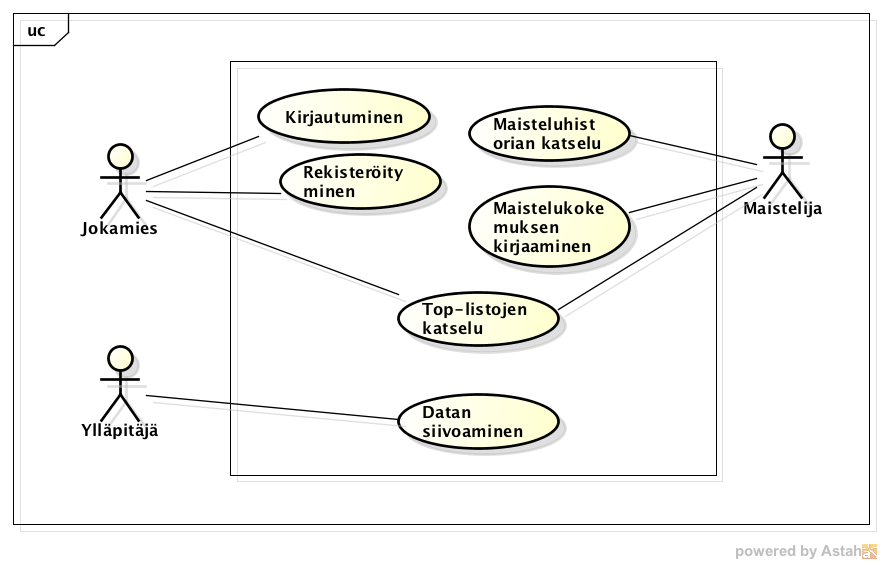
\includegraphics[width=12cm]{usecase}
  \caption{Käyttötapauskaavio}
  \label{fig:käyttötapaus}
\end{figure}

Kuvassa \ref{fig:käyttötapaus} on esitelty sovelluksen käyttäjäryhmät
ja käyttötapaukset. Käyttäjäryhmät ovat:

\begin{description}
\item[Jokamies] Jokamies on kuka tahansa, joka vierailee
  kahvipäiväkirjassa. Kaikki muut käyttäjäryhmät kuuluvat myös tähän
  käyttäjäryhmään.

\item[Maistelija] Maistelija on rekisteröity käyttäjä. Maistelija voi
  lisätä kahvipäiväkirjaan omia maistelukokemuksiaan.

\item[Ylläpitäjä] Ylläpitäjä pitää huolta siitä, että järjestelmään
  syötetty tieto on laadukasta.
\end{description}

\subsection{Jokamiehen käyttötapaukset}

\begin{description}
\item[Top-listojen katselu] Kuka tahansa voi katsella, mitkä kahvit ja
  mitkät kahvilat ovat saaneet parhaat arvosanat sovelluksen
  käyttäjien toimesta.
\end{description}

Muita käyttötapauksia: rekisteröityminen, kirjautuminen.

\subsection{Maistelijan käyttötapaukset}

\begin{description}
\item[Maistelukokemuksen lisääminen] Käyttäjä merkitsee muistiin mitä
  kahvia on juonut, antaa sille arvosanan ja lisää vapaamuotoiset
  muistiinpanot. Jos sovellus ei tunne kahvilaatua entuudestaan, se
  lisätään järjestelmään.

\item[Maisteluhistorian katselu] Käyttäjä pystyy selaamaan
  maistelukokemuksiaan ja saa yhteenvedon maisteluhistoriastaan.
\end{description}

\subsection{Ylläpitäjän käyttötapaukset}

\begin{description}
\item[Datan siivoaminen] Ylläpitäjä voi muokata lisättyjen
  kahvilaatujen tietoja ja tarvittaessa yhdistellä niitä. Esimerkki:
  kaksi käyttäjää ovat lisänneet saman kahvilaadun hieman eri
  nimellä. Ylläpitäjä käy yhdistämässä näiden tiedot.
\end{description}


\section{Järjestelmän tietosisältö}

Järjestelmän tietosisältöä korkealla tasolla kuvaa käsitekaavio
kuvassa \ref{fig:käsitekaavio}.

\begin{figure}[ht]
  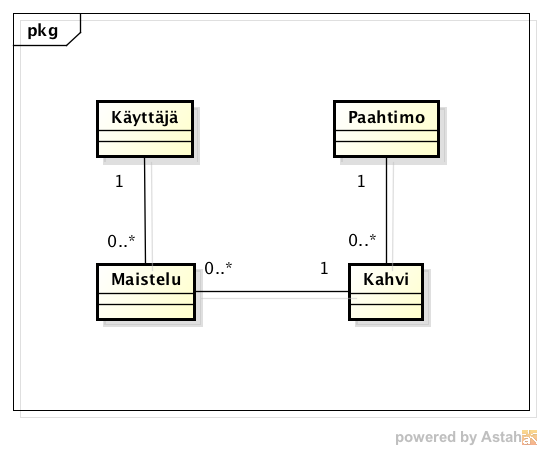
\includegraphics[width=12cm]{database}
  \caption{Käsitekaavio}
  \label{fig:käsitekaavio}
\end{figure}

\subsection{Tietokohde: Käyttäjä}

\begin{center}
\begin{tabularx}{\textwidth}{|X|X|X|}
\hline
Attribuutti & Arvojoukko & Kuvailu \\
\hline
Käyttäjänimi     & Merkkijono & Käyttäjän nimimerkki sovelluksessa. \\
Sähköpostiosoite & Merkkijono & Käyttäjän sähköposti osoite. Mahdollistaa kirjautumisen ja unohtuneen salasanan palauttamisen. \\
Liittymisaika    & Ajanhetki  & Milloin käyttäjätili on luotu. \\
Ylläpitäjyys     & Boolen arvo & Onko käyttäjällä ylläpito-oikeudet. \\
Salasana         & Merkkijono & Salasanan bcrypt-tiiviste. \\
\hline
\end{tabularx}
\end{center}

\subsection{Tietokohde: Paahtimo}

\begin{center}
\begin{tabularx}{\textwidth}{|X|X|X|}
\hline
Attribuutti & Arvojoukko & Kuvailu \\
\hline
Nimi & Merkkijono & Paahtimon nimi. \\
\hline
\end{tabularx}
\end{center}

Kullakin paahtimolla voi olla mielivaltainen määrä kahveja, mutta kukin kahvi voi kuulua vain yhdelle paahtimolle.

\subsection{Tietokohde: Kahvi}

\begin{center}
\begin{tabularx}{\textwidth}{|X|X|X|}
\hline
Attribuutti & Arvojoukko & Kuvailu \\
\hline
Nimi & Merkkijono & Kahvilaadun nimi. \\
\hline
\end{tabularx}
\end{center}

Kukin kahvi kuuluu aina täsmälleen yhdelle paahtimolle.

\subsection{Tietokohde: Maistelu}

\begin{center}
\begin{tabularx}{\textwidth}{ |X|X|X| }
\hline
Attribuutti & Arvojoukko & Kuvailu \\
\hline
Laatu & Merkkijono & Kahvin valmistustapa. \\
Sijainti & Merkkijono & Missä kahvi on nautittu. \\
Arvosana & Kokonaisluku, 1-5 & Yhdestä viiteen tähteä. \\
Muistiinpanot & Merkkijono & Käyttäjän apaamuotoiset muistiinpanot maistelusta. \\
Luontiaika & Ajanhetki & Milloin maistelukokemus on kirjattu. \\
\hline
\end{tabularx}
\end{center}

Kukin maistelukokemus kuuluu käyttäjälle, joka kokemuksen on
kirjannut. Kukin maistelu liittyy aina täsmälleen yhteen kahviin.


\section{Relaatiotietokantakaavio}

Sovelluksen tietokannan rakennetta kuvaa relaatiotietokantakaavio
\ref{fig:relaatiotietokantakaavio}.

\begin{figure}[ht]
  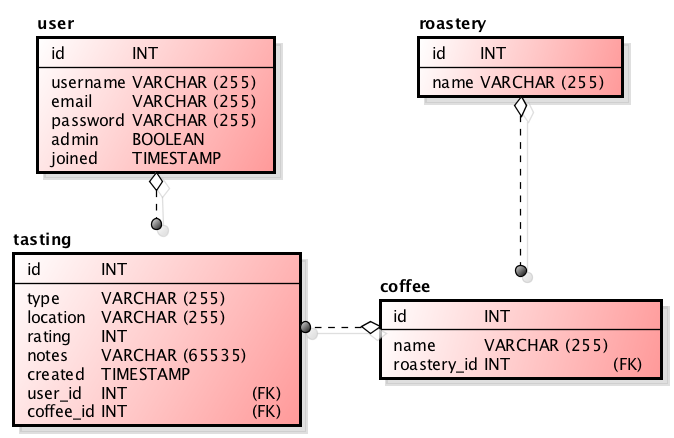
\includegraphics[width=12cm]{relational}
  \caption{Relaatiotietokantakaavio}
  \label{fig:relaatiotietokantakaavio}
\end{figure}


\section{Järjestelmän yleisrakenne}

Sovellus on tehty noudattaen MVC-mallia.
Vaikka Clojure tukeekin olio-ohjelmointia, se ei kannusta siihen.
Niinpä luokkien sijaan yhteen kokonaisuuteen kuuluvat funktiot on koottu nimiavaruuksiin.
MVC-malli ilmenee seuraavasti:

\begin{itemize}
    \item Näkymät on sijaitsevat
      \texttt{kahvipaivakirja.view}s-nimiavaruudessa. Ne on toteutettu
      Hiccup-kirjastolla, joka generoi HTML:ää
      Clojure-tietorakenteiden pohjalta. Kukin näkymä on
      Clojure-funktio, joka ottaa parametreikseen tarvitsemansa datan
      ja palauttaa näkymän HTML:ksi renderöitynä. Pohjanäkymä ja
      useilla sivuilla käytettyjä komponentteja on toteutettu
      Clojure-funktioina, jotka palauttavat Hiccup-yhteensopivaa
      dataa.

    \item Malleihin liittyvät funktiot sijaitsevat
      \texttt{kahvipaivakirja.models}-nimiavaruudessa. SQL-koodi on
      erikseen hakemistossa \texttt{src/sql}. Tietokantakutsut
      palauttavat Clojure-dataa.

    \item Kontrollerit on toteutettu
      \texttt{kahvipaivakirja.core}-nimiavaruudessa. Monimutkaisempia
      kontrollereja varten on omat funktionsa, yksinkertaisemmat
      kontrollerit on sisällytetty suoraan
      \texttt{defroutes}-reittitystauluun.
\end{itemize}


\subsection{Kirjautuminen ja sessiot}

Kirjautumisen toteutuksessa käytetään hyväksi
\href{https://github.com/cemerick/friend}{friend-kirjastoa}, joka
hoitaa käyttäjätietojen tarkistamisen ja session päivittämisen
kirjautumistietojen osalta. Käyttäjätiedot haetaan tietokannan
users-taulusta.

Sessioissa käytetään Ringin sessio-middlewarea, joka tallentaa sessiot
palvelimen muistiin. Käyttäjälle lähetetään
\texttt{ring-session}-niminen eväste, joka sisältää session
tunnuksen. Sessioiden tallentamisen muistiin varjopuolena on se, että
aina kun palvelin käynistetään uudestaan, esim. sovellusta
päivittäessä, sessiomuisti tyhjennetään.


\section{Käyttöliittymä}

Alustava sivukartta on esitetty kuvassa \ref{fig:sivukartta}.

\begin{figure}[ht]
  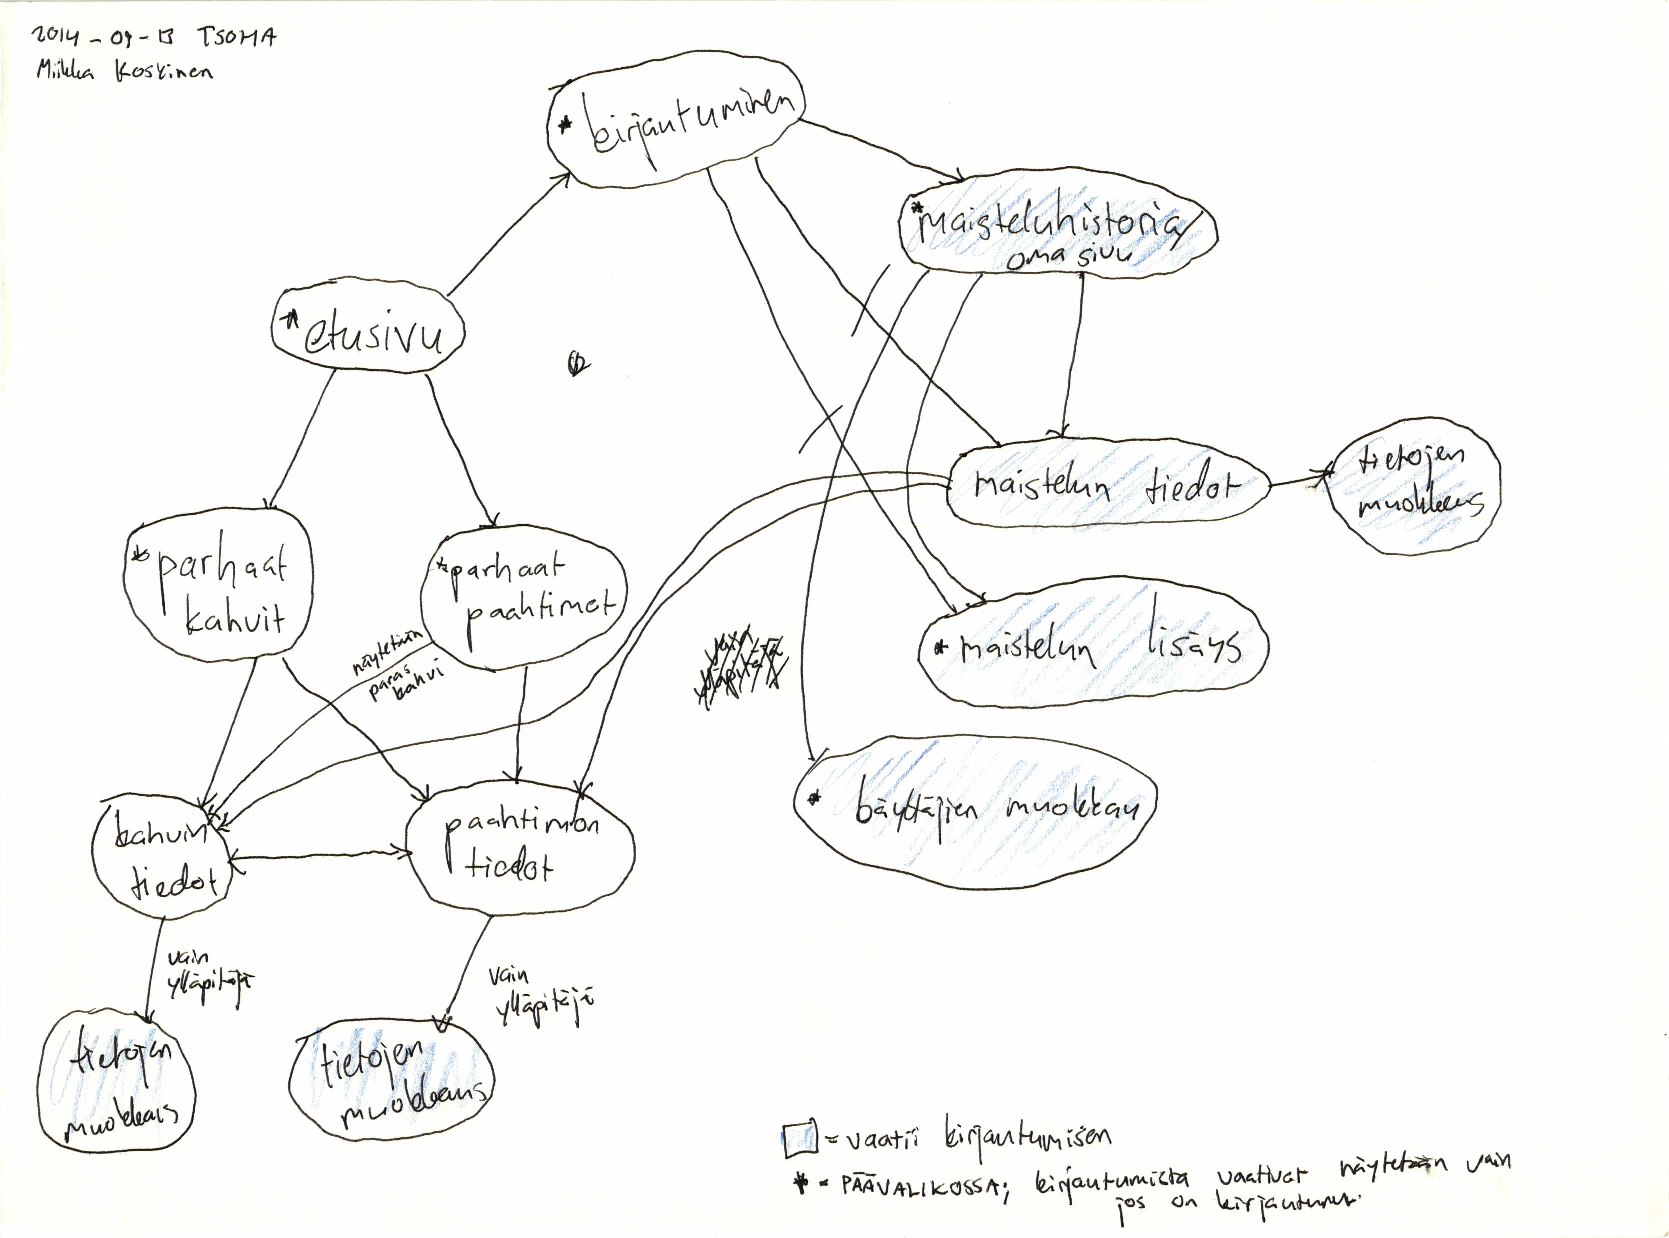
\includegraphics[width=12cm]{ui/sitemap}
  \caption{Alustava sivukartta}
  \label{fig:sivukartta}
\end{figure}

\section{Asennustiedot}

Sovelluksen asentamiseen tarvitaan Java, Make ja
\href{http://leiningen.org/}{Leiningen-projektinhallintatyökalu}. Leiningen
lataa ensimmäisellä ajokerralla automaattisesti kaikki tarvittavat
kirjastot \texttt{project.clj}-tiedoston mukaisesti, Clojure
mukaanlukien.

Sovellus käyttää tietokantana PostgreSQL:ia. Kehitys- ja
testauskäytössä voidaan käyttää HTTP-palvelimena Ring-kirjaston
palvelinta, joka käynistetään komennolla \texttt{lein ring
  server}. Tuotantokäytössä voidaan käyttää Tomcatia.

\subsection{Asennuksen vaiheet}

\begin{enumerate}
\item Asenna ja konfiguroi Java, PostgreSQL ja Tomcat.
\item Asenna Leiningen seuraamalla ohjeita osoitteessa \url{http://leiningen.org/#install}.
\item Luo asetustiedosto \path{~/.kahvipaivakirja.edn}. Asetukset on
  kuvattu osiossa \ref{sec:asetustiedosto}.
\item Alusta tietokanta komennolla \texttt{make reset-db}.
\item Luo WAR-tiedosto komennolla \texttt{make war}.
\item Kopio WAR-tiedosto Tomcatin \texttt{webapps}-hakemistoon.
\end{enumerate}

\subsection{Asetustiedosto}
\label{sec:asetustiedosto}

Sovelluksen tietokanta-asetukset tallennetaan EDN-muodossa tiedostoon
käyttäjän kotihakemistoon nimellä
\path{.kahvipaivakirja.edn}. Asetukset tallennetaan
clojure.java.jdbc-kirjaston tukemassa muodossa, joka on kuvattu
sivulla
\url{http://clojure-doc.org/articles/ecosystem/java_jdbc/home.html}. Esimerkiksi
jos käytetään paikallista PostgreSQL-tietokantaa \texttt{tietokanta}
käyttäjätunnuksella \texttt{kayttaja} ja salasanalla
\texttt{salasana}, asetukset näyttävät tältä:

\begin{lstlisting}[basicstyle=\ttfamily]
{:classname "org.postgresql.Driver"
 :subprotocol "postgresql"
 :subname "//localhost:5432/tietokanta"
 :user "kayttaja"
 :password "salasana"}
\end{lstlisting}

\section{Käynistys- ja käyttöohje}

Sovellus on asennettu \emph{users}-palvelimelle. Sovelluksen etusivu on osoitteessa \url{http://t-miikoski.users.cs.helsinki.fi/kahvipaivakirja/}. Testaamista varten on luotu seuraavat käyttäjätunnukset:

\begin{center}
\begin{tabularx}{\textwidth}{|X|X|}
\hline
Käyttäjänimi & Salasana \\
\hline
\texttt{Testaaja} & \texttt{kofeiini} \\
\texttt{Yllapitaja} & \texttt{kofeiini} \\
\hline
\end{tabularx}
\end{center}


\section{Testaus, tunnetut puutteet ja jatkokehitysideat}

Järjestelmää on testattu Firefox- ja Safari-selaimilla sekä iPhonen
Mobile Safari -selaimella. Mitään erityistä testausprosessia ei
ole. Normaalin käytön lisäksi olen testannut lisäksi manipuloimalla
lomakkeiden syötteitä selaimen kehitystyökaluilla. Automaattisia
testejä ei ole käytössä.

\subsection{Tunnetut puutteet ja kehityskohteet}

\begin{itemize}
\item Kahvin ja paahtimon voi yrittää yhdistää itsensä kanssa. Mitään
  ei tapahdu, jos niin tekee, mutta tämän ei pitäisi olla edes
  mahdollista käyttöliittymän kautta.
\item Kahvin ja paahtimon lisäämisen käyttöliittymä on jokseenkin
  kömpelö. Maistelunlisäyslomake voisi tarjota mahdollisuuden lisätä
  uusi kahvi ja paahtimo suoraan samalta sivulta.
\item Maistelukokemuksen katselusivu on samalla muokkaussivu. Tämä
  tuntuu rumalta.
\item Minkäänlaisia työkaluja käyttäjien lisäämiseen tai muokkaamiseen
  ei ole. Esimerkiksi jos käyttäjä unohtaa salasanansa, ylläpitäjän on
  asetettava se uudestaan ajamalla SQL-komentoja.
\item Yksikkötestejä ei ole. Niistä olisi ollut kehityksen aikana
  varmasti iloa.
\end{itemize}



\end{document}
